\chapter{Project Status}
\label{ch:project-status}

\graphicspath{{mainmatter/project-status/figures/}}

\section{Project Timeline}

A project timeline is given in \cref{fig:project-status:work-plan}. The project timeline consists of four phases (one preliminary) and seven milestones:

\bigskip
\begin{enumerate}[label=\textbf{Phase \arabic*.},start=0,leftmargin=2.5cm]
  \item \textbf{Early problem investigation.} Early investigation into the problem area, exploring potential aspects for research hypotheses to develop. The outcome is the first two chapters of this report (Milestone 1) and the early stages of a technical report attached in \cref{appx:tech-report}.
  \item \textbf{Develop initial framework.} Process of developing initial framework by mining developer forums (Stack Overflow) and designing and conduct our surveys. This maps to Experiment I (see \cref{ssec:research-methodology:experiments:2}). The outcome is an initial context-agnostic \gls{cis} \gls{api} documentation quality assessment framework (Milestone 3) and confirmation of candidature complete (Milestone 2). As ethics approval is required, the current draft Ethics Application is attached in \cref{appx:ethics}.
  \item \textbf{Validate initial framework.} Validating that the framework we develop in Phase 1 correctly reflects the needs of developers by trialing it in controlled observational studies. This maps to Experiment II (\cref{ssec:research-methodology:experiments:2}). The outcome is a framework that has been validated against developers (Milestone 4).
  \item \textbf{Finalise framework and thesis.} Implement any additional findings from the validation of Phase 2 into the framework, thereby finalising the framework (Milestone 5). Original contribution is the framework and therefore the thesis can be submitted (Milestone 6) and reviewed before the study is complete (Milestone 7).
\end{enumerate}

\begin{landscape}


\begin{figure}[p!]
  \vspace{-0.5cm}
  \centering
  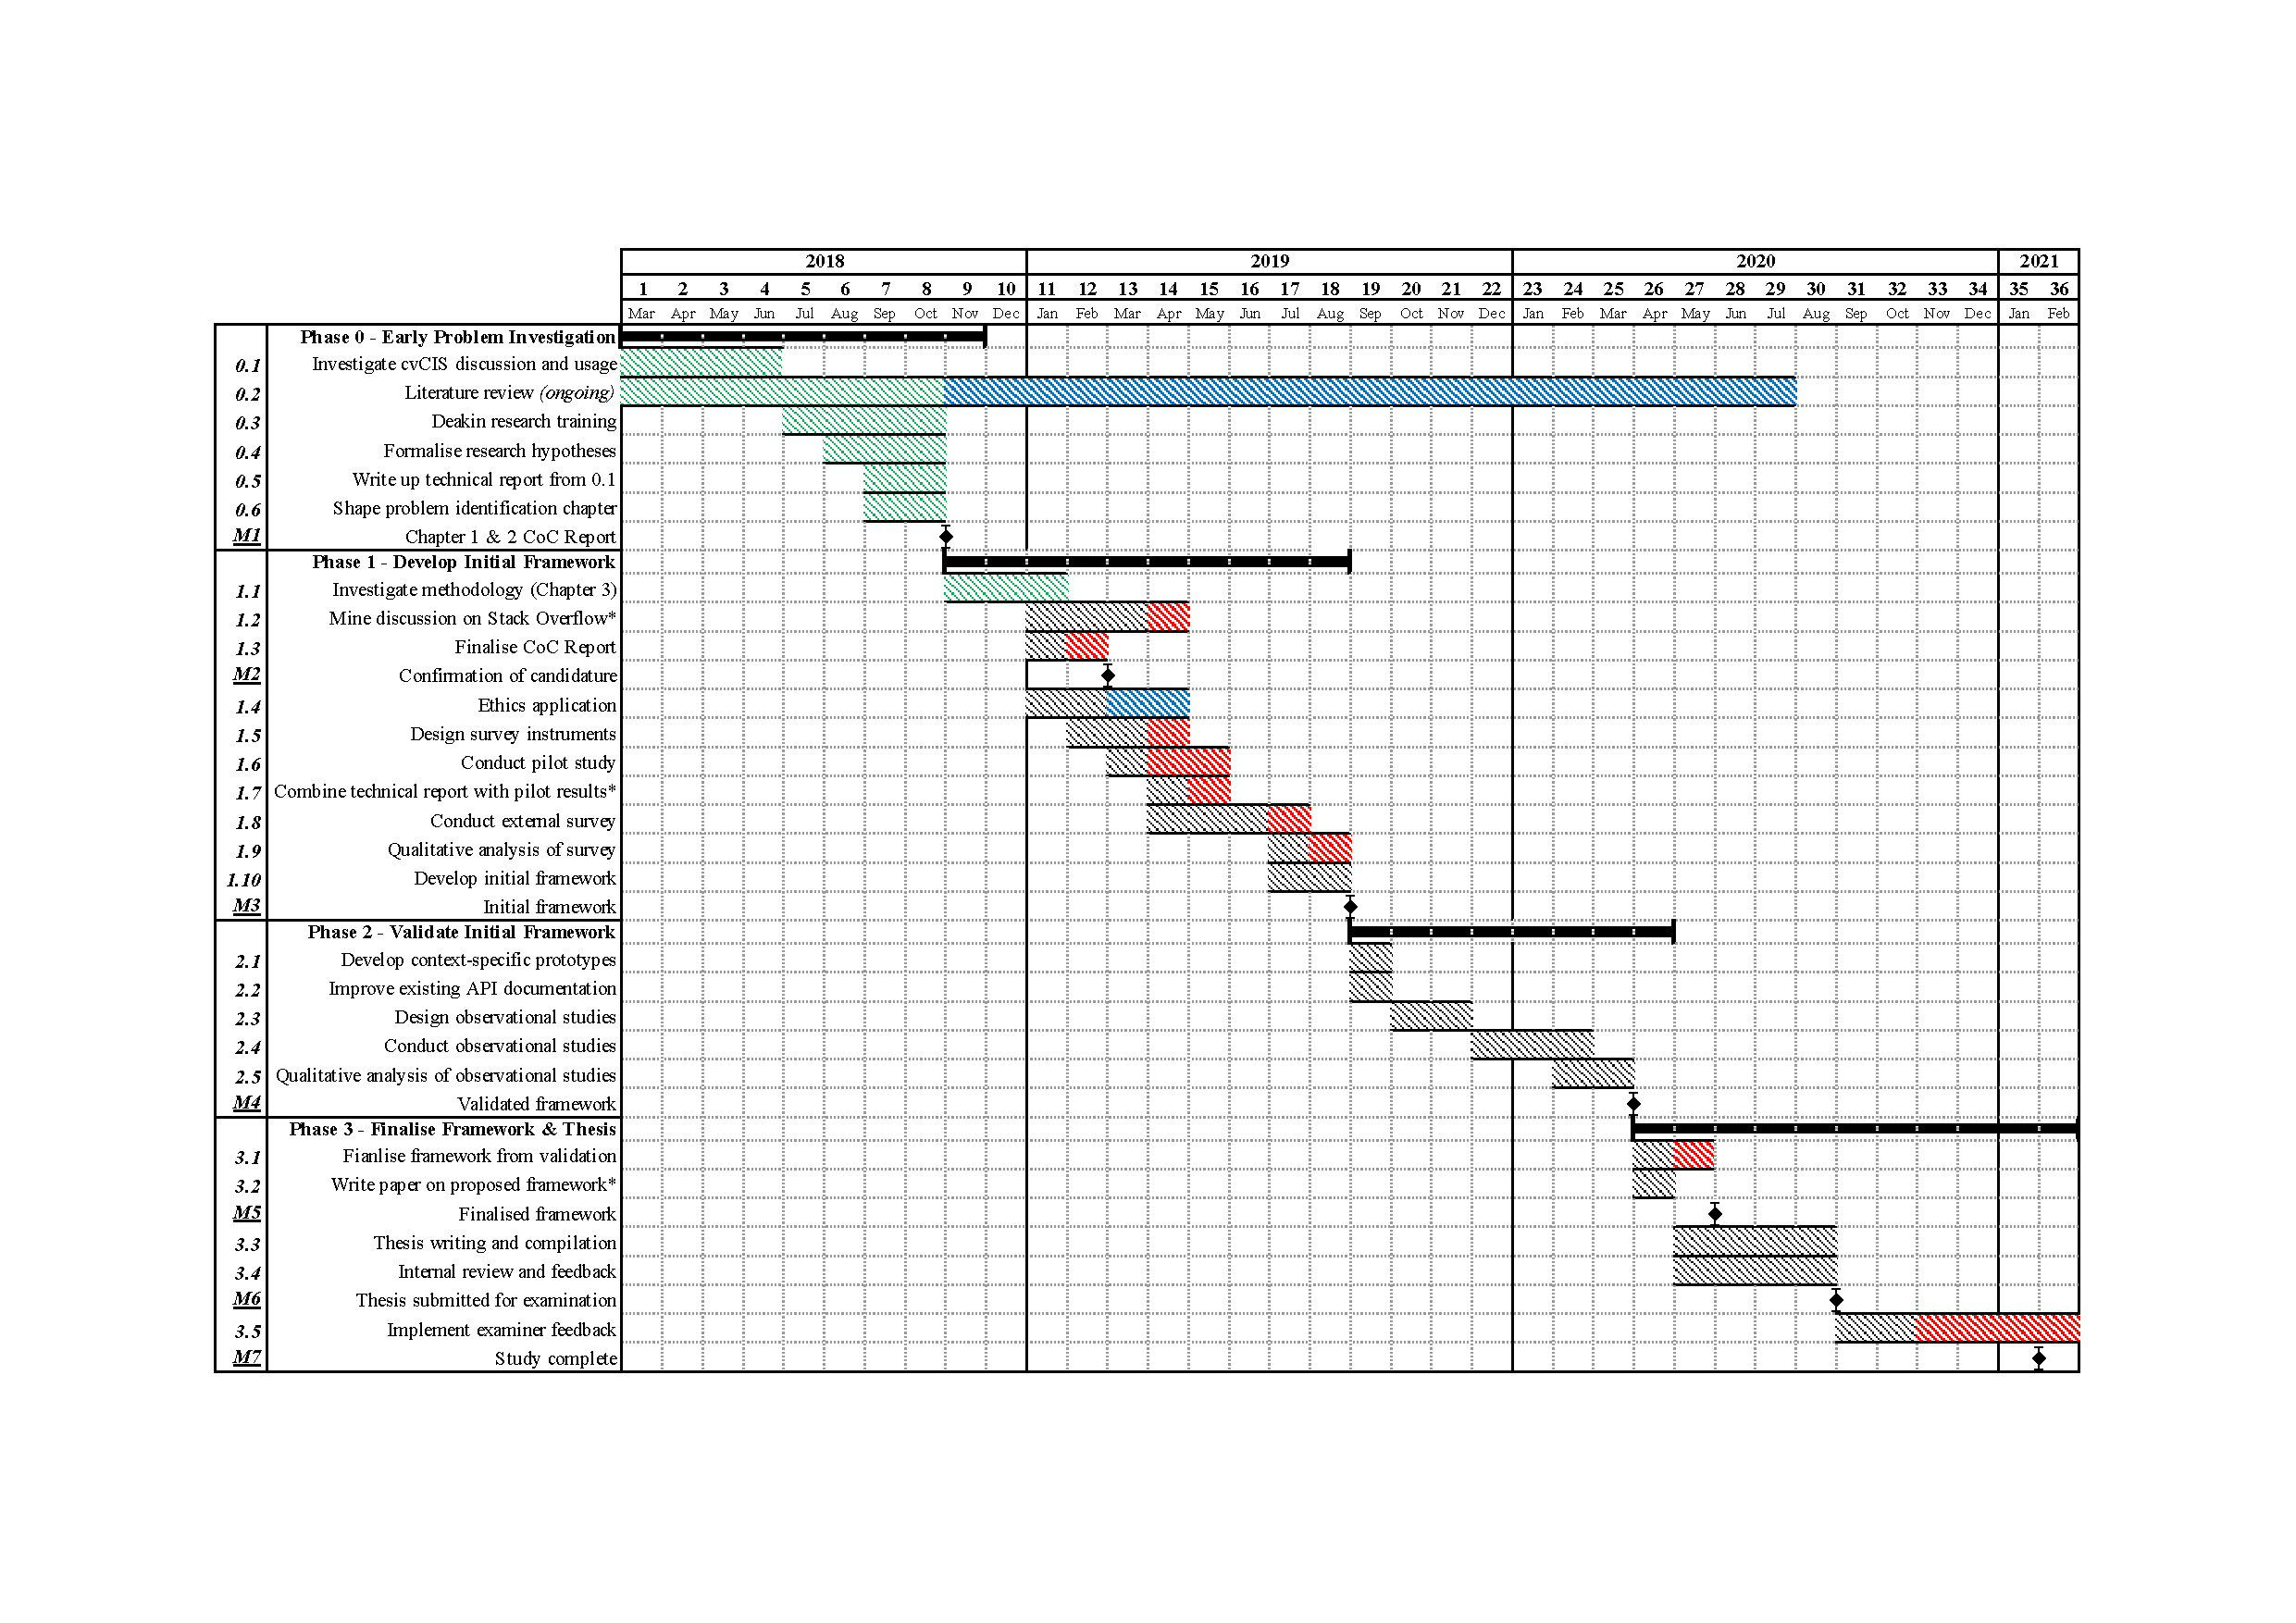
\includegraphics[width=\linewidth]{work-plan}
  \caption[PhD project timeline]{Project timeline. \\ \textit{\textbf{Key:} Green Bar = Completed Task; Grey Bar = Planned Task; Red Bar = Slack Time; Blue Bar = Ongoing Task; Thick Black Line = Phase Duration; Diamond = Milestone; Asterisk = Potential publications.}}
  \label{fig:project-status:work-plan}
\end{figure}
  
\end{landscape}

\begin{table}[p!]
\centering
\caption[Mapping of project tasks to research questions]{Mapping of project tasks (see \cref{fig:project-status:work-plan})  that address each of the research questions.}
\begin{tabular}{@{}l|l@{}}
\toprule
  % Heading
  \textbf{Research Question} &
  \textbf{Task \#} \\
  \midrule
    RQ1.1 & 0.1, 0.2, 1.2 \\
    RQ1.2 & 1.2, 1.6, 1.8, 1.10 \\
    RQ1.3 & 1.6, 1.8, 1.10 \\
    RQ2.1 & 2.1 \\
    RQ2.2 & 2.4, 2.5 \\
    RQ3.1 & 2.5 \\
    RQ3.2 & 2.5 \\
  \bottomrule
\end{tabular}
\end{table}


\begin{table}[p!]
\centering
\caption[Potential publications and venues]{Potential publications and respective targeted venues from outcomes of major bodies of work (see \cref{fig:project-status:work-plan}).}
\tablefit{
  \begin{tabular}{@{}ll|llll@{}}
  \toprule
    \textbf{Venue} &
    \textbf{Ranking} &
    \textbf{Task \#} &
    \textbf{Location} &
    \textbf{Submissions Due} &
    \textbf{Date} \\
    \midrule
      ESEC/FSE &
      A2 &
      1.2 &
      Tallinn, Estonia &
      20 Feb 2019 &
      26--30 Aug 2019
    \\
      ASE &
      A1 &
      1.2, 1.7 &
      San Diego, USA &
      6 May 2019 &
      11--15 Nov 2019
    \\
      CHI &
      A1 &
      1.2, 1.7 &
      Honolulu, USA &
      13 Sep 2019 &
      25--30 Apr 2020
    \\
      ICSE &
      A1 &
      1.7 &
      Seoul, South Korea &
      TBA &
      23--29 May 2020
    \\
      MSR &
      A1 &
      1.2, 1.7 &
      Seoul, South Korea &
      TBA &
      23--29 May 2020
    \\
      ICML &
      A1 &
      1.7 &
      Vienna, Austria &
      TBA &
      12--17 Jul 2020
    \\
      ICMLA &
      B2 &
      1.7, 3.2 &
      Copenhagen, Denmark &
      15 Nov 2020 &
      11--12 Jun 2021
    \\
    \midrule
    \thinrule
      TOSEM &
      N/A &
      1.2, 1.7; 3.2 &
      N/A &
      N/A &
      N/A
    \\
      IEEE Software &
      N/A &
      1.2, 1.7; 3.2 &    
      N/A &
      N/A &
      N/A
    \\
      TSE &
      N/A &
      1.2, 1.7; 3.2 &
      N/A &
      N/A &
      N/A
    \\
    \bottomrule
  \end{tabular}
}
\end{table}

\section{Completed Work}

\begin{itemize}
  \item \textbf{Ethics Application:} The progress of the ethics application (\cref{appx:ethics}) is well underway with the Low Risk Application Form filled out. Partial sections of the Plain Language Statement (PLS) is also complete but unattached with this document. We plan to submit ethics to Deakin SEBE HEAG within the next two weeks.
  \item \textbf{Technical Report:} Initial findings from our preliminary investigations of \glspl{cvcis} are attached within \cref{appx:tech-report}. We plan on triangulating these findings with further supporting results from Stack Overflow mining and survey research from our pilot study.
  \item \textbf{Progress on Thesis:} We have approached this report as the initial writeup of our thesis. We have substantially introduced our problem domain in \cref{ch:introduction}, a broad spectrum of literature in \cref{ch:background}, and our approach to the overall study in ]\cref{ch:research-methodology}. Whilst we aim to refine and enhance this work, this document will serve as a skeleton to the final thesis as we indicate below.
  \item \textbf{Stack Overflow Mining:} We have begun initial stages of our mining of Stack Overflow with preliminary results to be imported to qualitative analysis software such as NVivo.
\end{itemize}

\section{Proposed Chapters}

\begin{itemize}
  \item \textbf{Chapter 4 - \textit{Developer Opinions}:} This chapter maps to Experiment I (\cref{ssec:research-methodology:experiments:1}) by reporting directly related work regarding this experiment (i.e., surveys and interviews on nondeterministic systems, mining Stack Overflow for nondeterministic systems etc.), expanding on our methodology, and reporting our findings.
  \item \textbf{Chapter 5/6 - \textit{Proposed Framework}:} This chapter will introduce our proposed framework (initially the initial framework will be presented but the updated framework coming from our evaluation will be discussed). It will also describe the methodology by which we converted our qualitative and quantitative analyses to the framework. The order of the chapter is  to be determined.
  \item \textbf{Chapter 5/6 - \textit{Evaluation of Framework}:} This chapter maps to Experiment II (\cref{ssec:research-methodology:experiments:2}) and reports work directly related to evaluation of frameworks, expanding our methodology proposed and reporting our findings from the evaluation. The order of this chapter is to be determined.
  \item \textbf{Chapter 7 - \textit{Conclusions}:} This chapter will present concluding remarks of the study.
\end{itemize}


% Plan for thesis... Experiment 1 Chapter; Framework Chapter; Evaluation Chapter (Experiment 2); Conclusions

%\section{Descriptions of Completed Work}
%
%\subsection{Work completed from Phase 0}
%
%\paragraph{Task 0.1 Investigate \gls{cvcis} discussion and usage.} This 
%
%\section{Descriptions of Planned Work}
%
%\subsection{Planned work for Phase 1}
%
%\subsection{Planned work for Phase 2}
%
%\subsection{Planned work for Phase 3}
%\section{Intended Publications}